\documentclass[14pt,a4paper,oneside]{extbook}
\usepackage[utf8]{vietnam}
\usepackage{amsmath,amssymb,mathrsfs,fancyhdr,enumerate,multirow,makecell}
\usepackage{tkz-euclide,tikz-3dplot,tikz,tkz-tab}
\usetikzlibrary{arrows.meta,calc,intersections,angles,quotes,backgrounds,shapes.geometric,patterns,through,shadows,positioning}
\usepackage{yhmath}
\usepackage[top=0.7cm, bottom=0.7cm, left=1.0cm, right=1.0cm, headheight=16pt, headsep=3mm, footskip=5mm]{geometry}
\usepackage[hidelinks,unicode]{hyperref}
\usepackage{qrcode}
\usepackage[many]{tcolorbox}
\usepackage{fontawesome}

\pagestyle{fancy}
\fancyhf{}
\fancyhead[L]{\footnotesize\bfseries\color{teal!85!black}\faBook~SỔ TAY KIẾN THỨC TOÁN 5}
\fancyhead[R]{\footnotesize\bfseries\color{blue!85!black}Lớp Toán Thầy Lĩnh -- loptoanthaylinh.vn}
\fancyfoot[C]{\footnotesize\bfseries\color{gray!80!black}-- Sổ tay kiến thức: Bài 47. Mét khối --}
\renewcommand{\headrulewidth}{0.4pt}

\begin{document}

% --- BANNER TIÊU ĐỀ BÀI HỌC ---
\noindent
\begin{tcolorbox}[
  enhanced,
  colback=teal!8!white,
  colframe=teal!80!black,
  arc=3mm,
  boxrule=1.1pt,
  width=\linewidth,
  halign=center,
  top=2.2mm, bottom=2.2mm,
  left=3mm, right=3mm,
  drop fuzzy shadow
]
  {\large\bfseries\color{teal!95!black}\faBookmark\ BÀI 47. MÉT KHỐI}\\[2pt]
  {\scriptsize\color{black!75}\itshape Đơn vị m3, bảng quy đổi m3 - dm3 - cm3 và ứng dụng đo dung tích bể nước trên 1 trang A4}
\end{tcolorbox}

\vspace{3.2mm}
% --- KHỐI 1: ĐỊNH NGHĨA MÉT KHỐI ---
\noindent
\begin{minipage}[t]{0.56\textwidth}
  \begin{tcolorbox}[
    enhanced,
    title={\footnotesize\bfseries\color{white}\faCube\ 1. Khái niệm Mét khối ($\text{m}^3$)},
    colback=blue!2!white,
    colframe=blue!75!black,
    arc=2.5mm, boxrule=0.8pt, top=1.8mm, bottom=1.8mm, left=2.2mm, right=2.2mm
  ]
    \footnotesize
    $\bullet$ Là thể tích của \textbf{hình lập phương có cạnh dài $1\text{ m}$}.\\
    $\bullet$ Kí hiệu: \textbf{$\text{m}^3$}.\\
    $\bullet$ Thường dùng đo thể tích bể nước, phòng học, thùng container, khối đất, cát đá xây dựng.\\
    \begin{tcolorbox}[colback=white, colframe=blue!75!black, boxrule=0.5pt, arc=1.5mm, halign=center, top=1mm, bottom=1mm]
      {\scriptsize\bfseries\color{blue!90!black}$1\text{ m}^3 = 1\,000\text{ dm}^3 = 1\,000\text{ lít} = 1\,000\,000\text{ cm}^3$}
    \end{tcolorbox}
  \end{tcolorbox}
\end{minipage}%
\hfill
\begin{minipage}[t]{0.42\textwidth}
  \begin{tcolorbox}[
    enhanced,
    title={\footnotesize\bfseries\color{white}\faTint\ Quy đổi ra Lít},
    colback=teal!2!white,
    colframe=teal!75!black,
    arc=2.5mm, boxrule=0.8pt, top=1.8mm, bottom=1.8mm, left=2mm, right=2mm,
    halign=center
  ]
    \footnotesize
    $1\text{ m}^3 = 1\,000\text{ dm}^3$\\[2pt]
    $= \mathbf{1\,000\text{ lít nước}}$\\[3pt]
    {\tiny\color{teal!95!black}\bfseries Một khối nước bằng $1\,000$ lít nước}
  \end{tcolorbox}
\end{minipage}

\vspace{3mm}

% --- KHỐI 2: BẢNG TỔNG KẾT 3 ĐƠN VỊ ĐO THỂ TÍCH ---
\noindent
\begin{tcolorbox}[
  enhanced,
  title={\footnotesize\bfseries\color{white}\faTable\ 2. Bảng đối chiếu 3 đơn vị đo thể tích Tiểu học},
  colback=purple!2!white,
  colframe=purple!70!black,
  arc=2.5mm, boxrule=0.8pt, top=1.8mm, bottom=1.8mm, left=2.5mm, right=2.5mm
]
  \scriptsize
  \centering
  \begin{tabular}{|c|c|c|}
    \hline
    \textbf{Mét khối ($\text{m}^3$)} & \textbf{Đề-xi-mét khối ($\text{dm}^3$)} & \textbf{Xăng-ti-mét khối ($\text{cm}^3$)} \\ \hline
    $1\text{ m}^3 = 1\,000\text{ dm}^3$ & $1\text{ dm}^3 = 1\,000\text{ cm}^3 = \frac{1}{1000}\text{ m}^3$ & $1\text{ cm}^3 = \frac{1}{1000}\text{ dm}^3 = \frac{1}{1000000}\text{ m}^3$ \\ \hline
  \end{tabular}\\[3pt]
  {\tiny\color{purple!90!black}\bfseries Mỗi đơn vị thể tích gấp 1 000 lần đơn vị liền sau, và bằng $\frac{1}{1000}$ đơn vị liền trước. Mỗi cột ứng với ĐÚNG 3 CHỮ SỐ!}
\end{tcolorbox}

\vspace{3mm}

% --- KHỐI 3: SƠ ĐỒ TƯ DUY ---
\noindent
\begin{tcolorbox}[
  enhanced,
  title={\footnotesize\bfseries\color{white}\faSitemap\ Sơ đồ tư duy: Quy tắc bước nhảy $1\,000$ lần},
  colback=yellow!2!white,
  colframe=teal!85!black,
  arc=3mm, boxrule=0.9pt, top=1.8mm, bottom=1.8mm, left=1.5mm, right=1.5mm,
  halign=center
]
  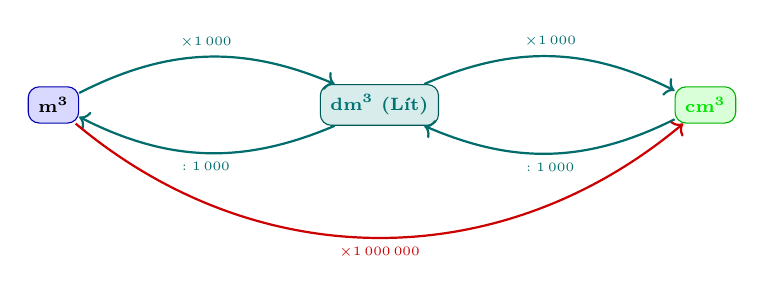
\begin{tikzpicture}[
    scale=0.92,
    every node/.style={transform shape},
    b1/.style={rectangle, rounded corners=4pt, fill=blue!15, draw=blue!70!black, font=\bfseries\scriptsize, inner sep=4pt},
    b2/.style={rectangle, rounded corners=4pt, fill=teal!15, draw=teal!70!black, text=teal!90!black, font=\bfseries\scriptsize, inner sep=4pt},
    b3/.style={rectangle, rounded corners=4pt, fill=green!15, draw=green!70!black, text=green!90!black, font=\bfseries\scriptsize, inner sep=4pt}
  ]
    \node[b1] (m) at (-4.5, 0) {$\mathbf{m^3}$};
    \node[b2] (dm) at (0, 0) {$\mathbf{dm^3}$ (Lít)};
    \node[b3] (cm) at (4.5, 0) {$\mathbf{cm^3}$};

    \draw[teal!85!black, thick, ->] (m) to[bend left=25] node[above, font=\tiny\bfseries] {$\times 1\,000$} (dm);
    \draw[teal!85!black, thick, ->] (dm) to[bend left=25] node[below, font=\tiny\bfseries] {$: 1\,000$} (m);
    \draw[teal!85!black, thick, ->] (dm) to[bend left=25] node[above, font=\tiny\bfseries] {$\times 1\,000$} (cm);
    \draw[teal!85!black, thick, ->] (cm) to[bend left=25] node[below, font=\tiny\bfseries] {$: 1\,000$} (dm);
    \draw[red!80!black, thick, ->] (m) to[bend right=40] node[below, font=\tiny\bfseries] {$\times 1\,000\,000$} (cm);
  \end{tikzpicture}
\end{tcolorbox}

\vspace{3mm}

% --- KHỐI 4: PHƯƠNG PHÁP 3 CHỮ SỐ & BẪY TRẮC NGHIỆM ---
\noindent
\begin{minipage}[t]{0.54\textwidth}
  \begin{tcolorbox}[
    enhanced,
    title={\footnotesize\bfseries\color{white}\faBolt\ Phương pháp 3 chữ số mỗi hàng},
    colback=green!3!white,
    colframe=green!60!black,
    arc=2.5mm, boxrule=0.8pt, top=1.8mm, bottom=1.8mm, left=2.2mm, right=2.2mm
  ]
    \footnotesize
    Viết $5\text{ m}^3\ 8\text{ dm}^3$ ra $\text{m}^3$:\\
    \centering
    \begin{tabular}{|c|c|c|}
      \hline
      $\text{m}^3$ & $\text{dm}^3$ & $\text{cm}^3$ \\ \hline
      $5$ & $0\ 0\ 8$ & $0\ 0\ 0$ \\ \hline
    \end{tabular}\\[2pt]
    $\Rightarrow 5\text{ m}^3\ 8\text{ dm}^3 = \mathbf{5,008\text{ m}^3}$.\\
    Hàng $\text{dm}^3$ có số $8$ đứng một mình $\rightarrow$ Thêm hai chữ số $0$ phía trước.
  \end{tcolorbox}
\end{minipage}%
\hfill
\begin{minipage}[t]{0.44\textwidth}
  \begin{tcolorbox}[
    enhanced,
    title={\footnotesize\bfseries\color{white}\faExclamationTriangle\ Mẹo tránh bẫy trắc nghiệm},
    colback=red!2!white,
    colframe=red!70!black,
    arc=2.5mm, boxrule=0.8pt, top=1.8mm, bottom=1.8mm, left=2.2mm, right=2.2mm
  ]
    \footnotesize
    $\bullet$ Đổi $1\text{ m}^3$ ra $\text{cm}^3$: Nhớ là \textbf{$1\,000\,000\text{ cm}^3$} ($6$ chữ số $0$, không phải $10\,000$).\\
    $\bullet$ Phân biệt: Độ dài gấp $10$, Diện tích gấp $100$, Thể tích gấp $1\,000$.
  \end{tcolorbox}
\end{minipage}

\end{document}
